% !TeX program = xelatex
\documentclass[UTF8,zihao=-4,fontset=fandol]{ctexart}
\usepackage[a4paper,left=21mm,right=21mm,top=17mm,bottom=19mm,footskip=9mm]{geometry}
\usepackage{fontspec,graphicx,xcolor,tikz,caption,fancyhdr}
\usepackage[unicode]{hyperref}

\setmainfont{TeX Gyre Pagella}
\setsansfont{TeX Gyre Heros}
\graphicspath{{figures/}}
\definecolor{ink}{HTML}{192E43}
\definecolor{sea}{HTML}{215C80}
\definecolor{quiet}{HTML}{415769}
\newcommand{\repoURL}{https://github.com/ZHT1235456/Three-js-USV-by-GPT-6.2-Astra}
\hypersetup{
  pdftitle={基于GPT-6.2 Astra制作的水面无人艇},
  pdfauthor={朱华天，GPT-6.2 Astra},
  pdflang={zh-CN},colorlinks=true,urlcolor=sea,linkcolor=sea
}
\ctexset{section={
  format=\Large\sffamily\heiti\bfseries\color{ink},
  beforeskip=12pt,afterskip=6pt
}}
\captionsetup{font={small,color=quiet},labelfont={bf,color=sea},
  labelsep=quad,justification=raggedright,singlelinecheck=false,hypcap=false,skip=6pt}
\setlength{\parindent}{0pt}
\setlength{\parskip}{3pt}
\pagestyle{fancy}
\fancyhf{}
\renewcommand{\headrulewidth}{0pt}
\fancyfoot[R]{\small\color{quiet}第 \thepage\ 页}

\title{基于GPT-6.2 Astra制作的水面无人艇}
\author{朱华天，GPT-6.2 Astra}
\date{2026年11月18日}
\makeatletter
\renewcommand{\maketitle}{%
  {\color{ink}\heiti\bfseries\fontsize{24}{32}\selectfont\@title\par}
  \vspace{2mm}
  {\@author\par}
  {\small\color{quiet}\@date\par}
  {\small\sffamily\href{\repoURL}{\repoURL}\par}
  \vspace{2mm}
}
\makeatother

\begin{document}
\maketitle

这艘蓝白单体无人艇用 Three.js 建模。艇艏上扬，低矮的设备舱居中，
仪器桅杆立在舱盖上。蓝色饰带从艉部沿舷侧收向艇艏，勾出白色船壳的轮廓。

\addvspace{7pt}
\begin{minipage}{\linewidth}
  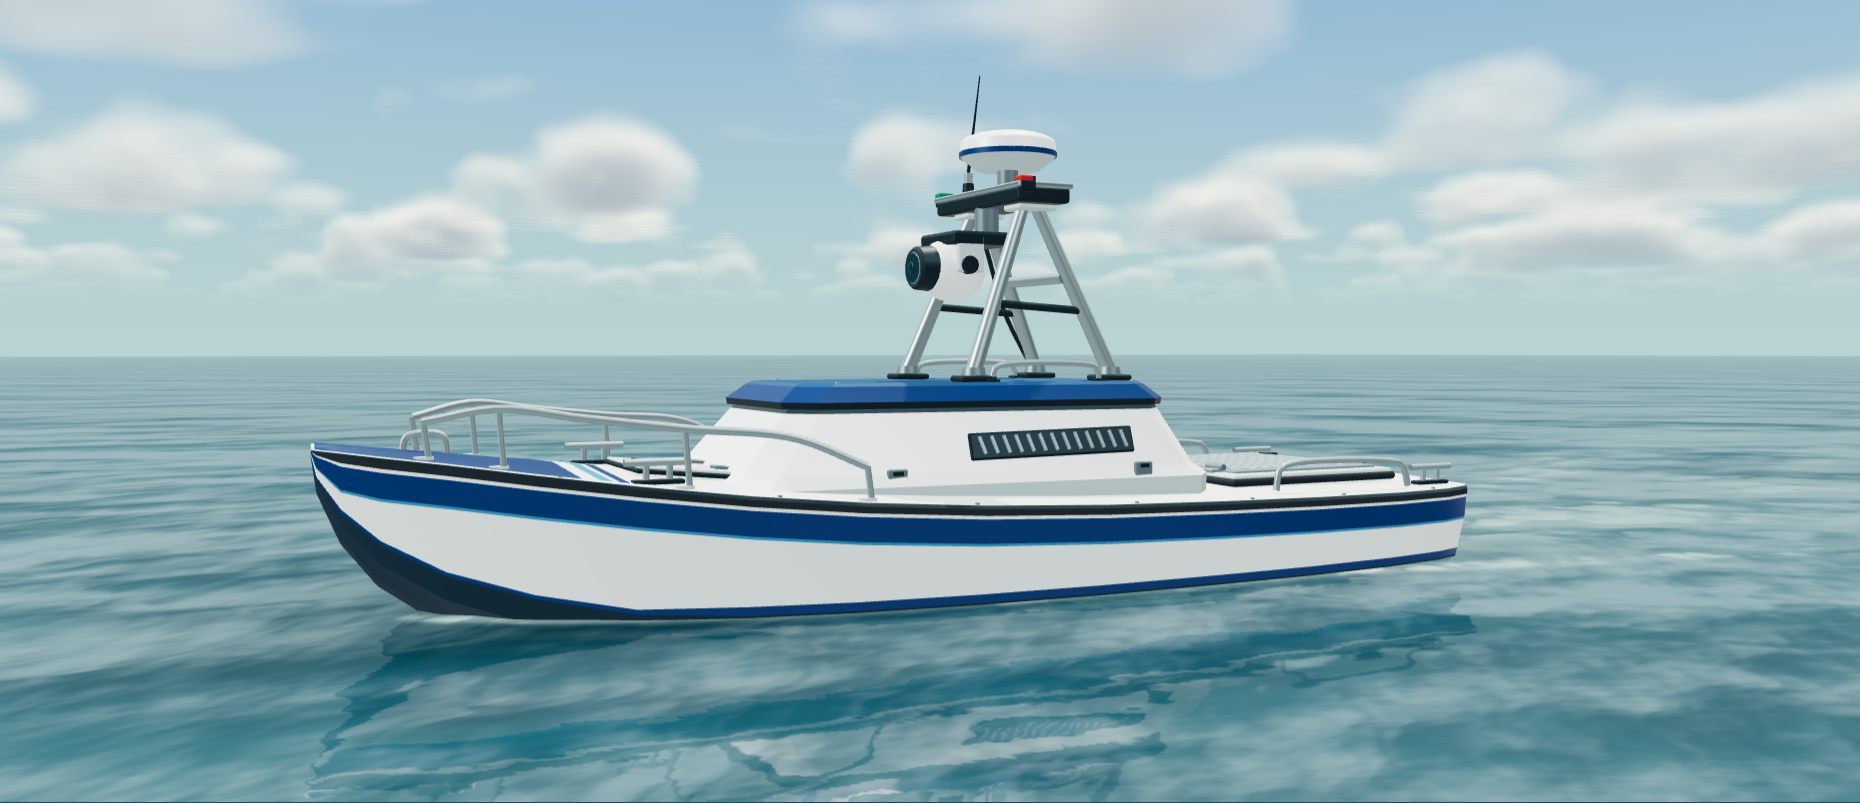
\includegraphics[width=\linewidth]{vessel.png}
  \captionof{figure}{水面上的整艇侧视。艇艏在左，艉部的开放甲板在右。}
\end{minipage}

\section*{从横剖面放样船壳}
船壳由一组沿艇长布置的横剖面放样而成。每个剖面以半宽、舷缘高度和龙骨高度
确定一侧轮廓，再沿中纵面镜像得到另一侧。相邻剖面的对应顶点连接成三角面，
在艇艏逐渐收尖，在艇艉以横向封板收尾。下图的剖线取自成品模型的船壳网格。

\addvspace{7pt}
\begin{minipage}{\linewidth}
  \resizebox{\linewidth}{!}{% Geometry projected from the Shallow-V hull mesh in the project GLB.
\begin{tikzpicture}[x=1mm,y=1mm,line join=round,line cap=round,font=\small\sffamily]
  \path[use as bounding box] (0,0) rectangle (168,57);
  \fill[sea!4] (0,0) rectangle (168,57);
  \draw[sea!24,line width=.3pt] (110,5) -- (110,52);
  \node[anchor=west,text=ink] at (4,51) {甲板外缘俯视};
  \node[anchor=west,text=ink] at (113,51) {A--A 横剖面};
  \fill[sea!9] (12.40,39.92) --
    (13.62,41.10) --
    (16.77,42.12) --
    (23.04,43.15) --
    (32.16,43.87) --
    (41.66,44.10) --
    (51.92,44.06) --
    (61.80,43.61) --
    (70.54,42.62) --
    (77.76,41.02) --
    (84.60,38.59) --
    (90.68,35.63) --
    (95.81,32.62) --
    (99.61,30.12) --
    (101.89,28.44) --
    (103.30,27.30) --
    (103.60,27.04) --
    (103.60,26.96) --
    (103.30,26.70) --
    (101.89,25.56) --
    (99.61,23.88) --
    (95.81,21.38) --
    (90.68,18.37) --
    (84.60,15.41) --
    (77.76,12.98) --
    (70.54,11.38) --
    (61.80,10.39) --
    (51.92,9.94) --
    (41.66,9.90) --
    (32.16,10.13) --
    (23.04,10.85) --
    (16.77,11.88) --
    (13.62,12.90) --
    (12.40,14.08) -- cycle;
\draw[sea!42,line width=.33pt] (13.62,41.10) -- (13.62,12.90);
\draw[sea!42,line width=.33pt] (16.77,42.12) -- (16.77,11.88);
\draw[sea!42,line width=.33pt] (23.04,43.15) -- (23.04,10.85);
\draw[sea!42,line width=.33pt] (32.16,43.87) -- (32.16,10.13);
\draw[sea!42,line width=.33pt] (41.66,44.10) -- (41.66,9.90);
\draw[sea!42,line width=.33pt] (61.80,43.61) -- (61.80,10.39);
\draw[sea!42,line width=.33pt] (70.54,42.62) -- (70.54,11.38);
\draw[sea!42,line width=.33pt] (77.76,41.02) -- (77.76,12.98);
\draw[sea!42,line width=.33pt] (84.60,38.59) -- (84.60,15.41);
\draw[sea!42,line width=.33pt] (90.68,35.63) -- (90.68,18.37);
\draw[sea!42,line width=.33pt] (95.81,32.62) -- (95.81,21.38);
\draw[sea!42,line width=.33pt] (99.61,30.12) -- (99.61,23.88);
\draw[sea!42,line width=.33pt] (101.89,28.44) -- (101.89,25.56);
\draw[sea!42,line width=.33pt] (103.30,27.30) -- (103.30,26.70);
\draw[sea,dashed,line width=.4pt] (8.60,27.00) -- (106.64,27.00);
\draw[ink,line width=.8pt] (12.40,39.92) --
    (13.62,41.10) --
    (16.77,42.12) --
    (23.04,43.15) --
    (32.16,43.87) --
    (41.66,44.10) --
    (51.92,44.06) --
    (61.80,43.61) --
    (70.54,42.62) --
    (77.76,41.02) --
    (84.60,38.59) --
    (90.68,35.63) --
    (95.81,32.62) --
    (99.61,30.12) --
    (101.89,28.44) --
    (103.30,27.30) --
    (103.60,27.04) --
    (103.60,26.96) --
    (103.30,26.70) --
    (101.89,25.56) --
    (99.61,23.88) --
    (95.81,21.38) --
    (90.68,18.37) --
    (84.60,15.41) --
    (77.76,12.98) --
    (70.54,11.38) --
    (61.80,10.39) --
    (51.92,9.94) --
    (41.66,9.90) --
    (32.16,10.13) --
    (23.04,10.85) --
    (16.77,11.88) --
    (13.62,12.90) --
    (12.40,14.08) -- cycle;
\draw[sea,line width=1.15pt] (51.92,46.00) -- (51.92,8.00);
  \node[anchor=south,text=sea,inner sep=1pt,font=\footnotesize\bfseries] at (51.92,46.38) {A};
  \node[anchor=north,text=sea,inner sep=1pt,font=\footnotesize\bfseries] at (51.92,7.62) {A};
  \node[anchor=west,text=quiet,font=\footnotesize] at (3,13) {艉};
  \node[anchor=east,text=quiet,font=\footnotesize] at (107,19) {艏};
\draw[draw=ink,fill=sea!10,line width=.85pt] (139.00,35.02) --
    (160.29,34.45) --
    (160.29,34.45) --
    (160.55,34.16) --
    (160.55,33.58) --
    (160.38,33.25) --
    (160.12,31.09) --
    (160.06,30.85) --
    (159.16,26.96) --
    (158.99,26.19) --
    (158.35,23.42) --
    (155.60,21.08) --
    (145.68,18.75) --
    (139.00,17.74) --
    (132.32,18.75) --
    (122.40,21.08) --
    (119.65,23.42) --
    (119.01,26.19) --
    (118.84,26.96) --
    (117.94,30.85) --
    (117.88,31.09) --
    (117.62,33.25) --
    (117.45,33.58) --
    (117.45,34.16) --
    (117.71,34.45) --
    (117.71,34.45) -- cycle;
\draw[sea!65,densely dashed,line width=.35pt] (139,13) -- (139,39);
\draw[sea!75,line width=.45pt] (139.00,17.74) -- (135,12) -- (129,12);
  \node[anchor=east,inner sep=1pt,text=quiet,font=\footnotesize] at (129,12) {龙骨};
\draw[sea!75,line width=.45pt] (160.29,34.45) -- (157,40) -- (151,40);
  \node[anchor=east,inner sep=1pt,text=quiet,font=\footnotesize] at (151,40) {舷缘};
\end{tikzpicture}
}
  \captionof{figure}{左图标出了各横剖面的位置。沿 A--A 剖开，可见艇底从中线龙骨向两舷抬升，形成浅 V 形。}
\end{minipage}

\newpage
\section*{甲板与设备舱}
设备舱由带切角的多层轮廓叠合而成，上层轮廓向内收，形成倾斜的舱壁。
蓝色舱盖略微挑出，边缘露出一圈深色密封边。艏部护栏沿舷侧收窄，
支柱脚点随甲板起伏。艉部检修盖上的平行防滑筋和铰链则用独立几何体拼装。

\addvspace{7pt}
\begin{minipage}{\linewidth}
  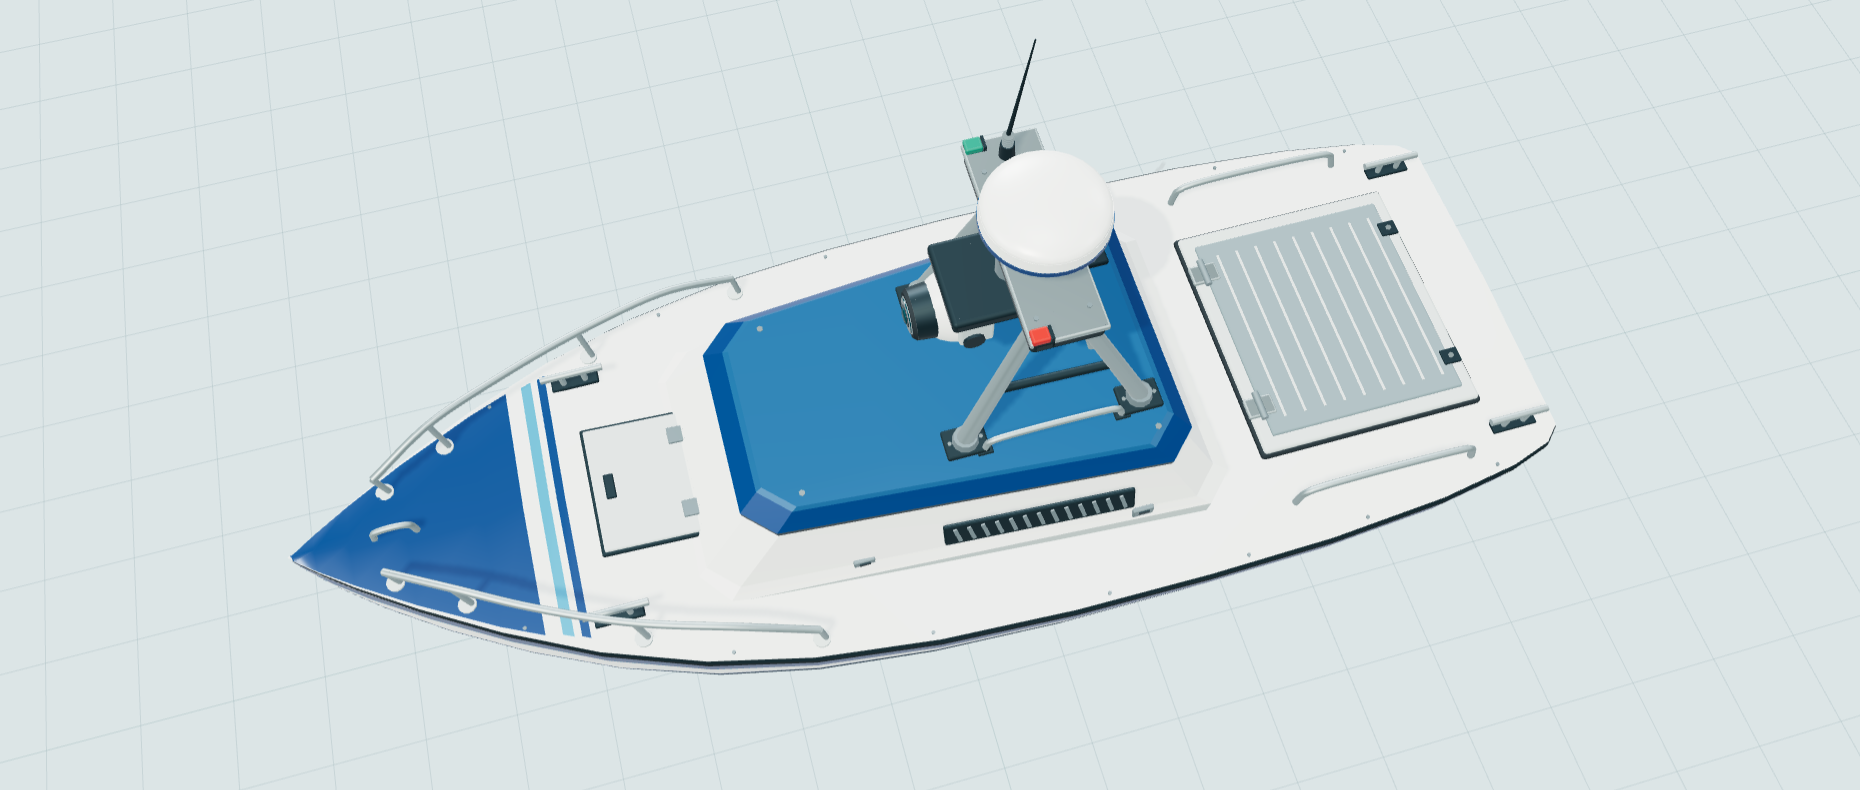
\includegraphics[width=\linewidth]{deck.png}
  \captionof{figure}{从斜上方观察甲板。由艏至艉依次可见前检修口、蓝色设备舱盖和带防滑筋的艉部检修盖。}
\end{minipage}

\section*{桅杆与水下组件}
桅杆的斜撑由逐渐收细的圆杆构成，顶部横梁把 GNSS 天线与前视相机分置在上下两侧。
艉部的三叶螺旋桨从桨毂向外逐段生成，叶片沿半径改变宽度和扭角。
后方的舵叶由沿舵杆高度排列的翼形截面连接成形，底端收窄。

\addvspace{7pt}
\noindent
\begin{minipage}[t]{.484\linewidth}
  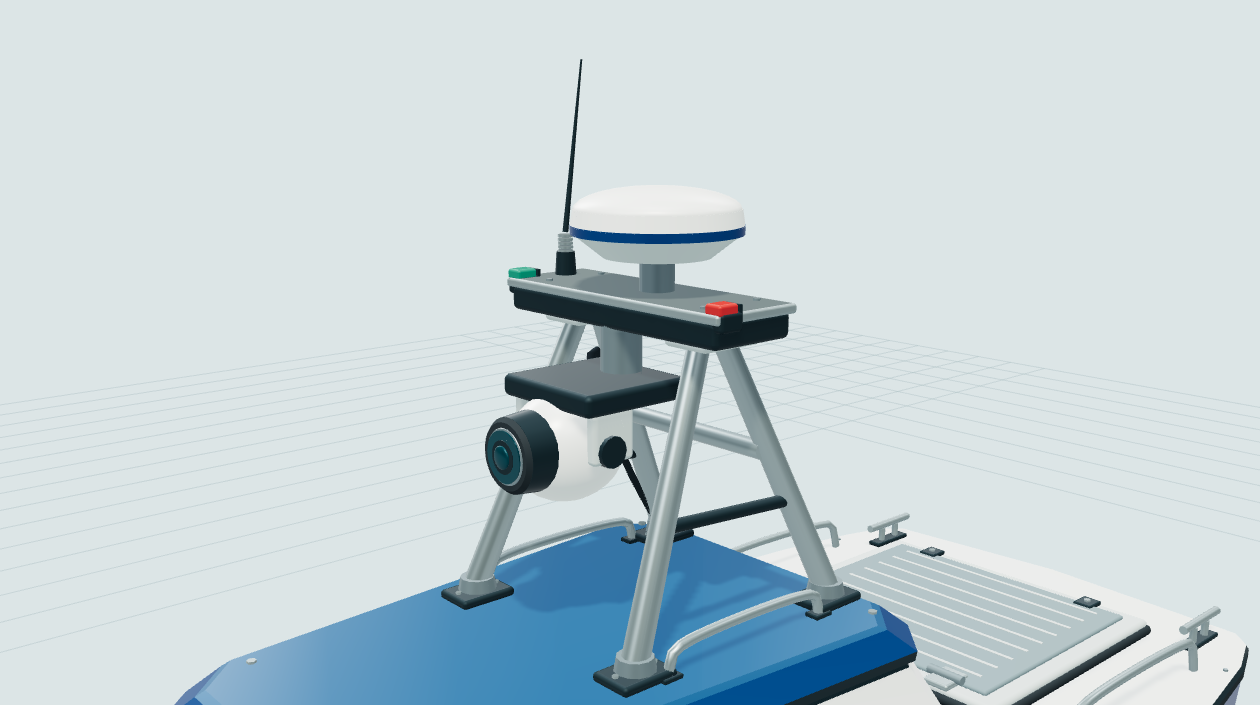
\includegraphics[width=\linewidth]{mast.png}
  \captionof{figure}{桅杆总成。白色天线罩在横梁上方，相机的支架和镜筒位于下方。}
\end{minipage}\hfill
\begin{minipage}[t]{.484\linewidth}
  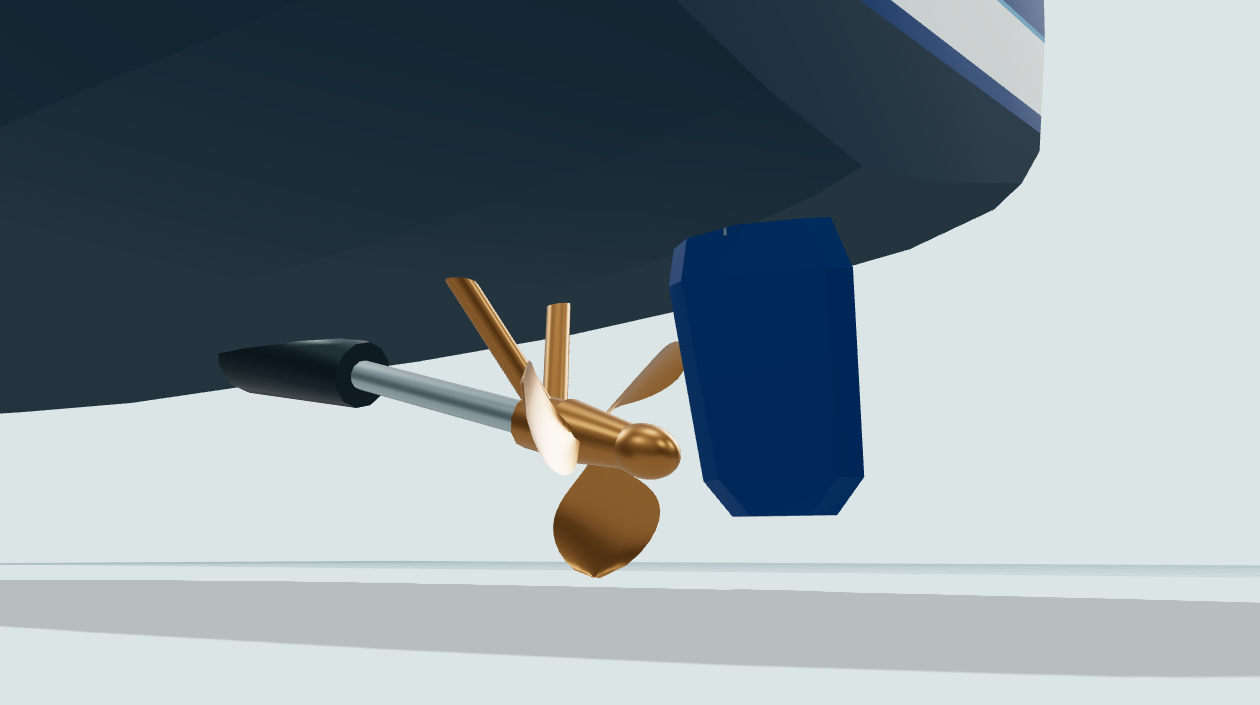
\includegraphics[width=\linewidth]{drive.png}
  \captionof{figure}{水线下的装配关系。倾斜的桨轴连接铜色螺旋桨，蓝色舵叶位于桨后。}
\end{minipage}

\addvspace{7pt}
固定零件按所属组件与材质合并。螺旋桨和舵叶各自保留独立节点及局部转轴，
因此把 GLB 船模导入三维编辑器后，仍可分别绕桨轴旋转桨叶、绕舵杆偏转舵叶。
\end{document}
